%
% 6.006 problem set 3 solutions template
%
\documentclass[12pt,twoside]{article}

\newcommand{\name}{}

\usepackage{amssymb}
\usepackage{amsmath}
\usepackage{graphicx}
\usepackage{latexsym}
\usepackage{times,url}
\usepackage{cprotect}
\usepackage{listings}
\usepackage{graphicx}
\usepackage[table]{xcolor}
\usepackage[letterpaper]{geometry}
\usepackage{tikz-qtree}
\usepackage{enumerate}

\newcommand{\profs}{Instructors: Zachary Abel, Erik Demaine, Jason Ku}
\newcommand{\subj}{6.006}
\newcommand{\ttt}[1]{{\tt\small #1}}

\definecolor{dkgreen}{rgb}{0,0.6,0}
\definecolor{gray}{rgb}{0.5,0.5,0.5}
\definecolor{mauve}{rgb}{0.58,0,0.82}

\lstset{
  language=Python,
  aboveskip=1pc,
  belowskip=1pc,
  basicstyle={\footnotesize\ttfamily},
  numbers=left,
  showstringspaces=false,
  numberstyle=\tiny\color{gray},
  keywordstyle=\color{blue},
  commentstyle=\color{dkgreen},
  stringstyle=\color{mauve},
}

\tikzset{
  % every node/.style={minimum width=2em,draw,circle},
  % level 1/.style={sibling distance=2cm},
  level distance=1cm,
  edge from parent/.style=
  {draw,edge from parent path={(\tikzparentnode) -- (\tikzchildnode)}},
}

\newif\ifHideSolutions
\newcommand{\solution}[1]{\color{dkgreen}\textbf{Solution: }#1\color{black}}
\newcommand{\rubric}[1]{\color{dkgreen}{\bf Rubric:} #1\color{black}}

% \HideSolutionsfalse
% \ifHideSolutions
%   \renewcommand{\solution}[1]{}
%   \renewcommand{\rubric}[1]{}
% \fi

\newlength{\toppush}
\setlength{\toppush}{2\headheight}
\addtolength{\toppush}{\headsep}

\newcommand{\htitle}[2]{\noindent\vspace*{-\toppush}\newline\parbox{6.5in}
{\textit{Introduction to Algorithms: 6.006}\hfill\name\newline
Massachusetts Institute of Technology \hfill #2\newline
\profs\hfill #1 \vspace*{-.5ex}\newline
\mbox{}\hrulefill\mbox{}}\vspace*{1ex}\mbox{}\newline
\begin{center}{\Large\bf #1}\end{center}}

\newcommand{\handout}[2]{\thispagestyle{empty}
 \markboth{#1}{#1}
 \pagestyle{myheadings}\htitle{#1}{#2}}

\newcommand{\lecture}[3]{\thispagestyle{empty}
 \markboth{Lecture #1: #2}{Lecture #1: #2}
 \pagestyle{myheadings}\htitle{Lecture #1: #2}{#3}}

\newcommand{\htitlewithouttitle}[2]{\noindent\vspace*{-\toppush}\newline\parbox{6.5in}
{\textit{Introduction to Algorithms}\hfill#2\newline
Massachusetts Institute of Technology \hfill 6.006\newline
\profs\hfill Handout #1\vspace*{-.5ex}\newline
\mbox{}\hrulefill\mbox{}}\vspace*{1ex}\mbox{}\newline}

\newcommand{\handoutwithouttitle}[2]{\thispagestyle{empty}
 \markboth{Handout \protect\ref{#1}}{Handout \protect\ref{#1}}
 \pagestyle{myheadings}\htitlewithouttitle{\protect\ref{#1}}{#2}}

\newcommand{\exam}[2]{% parameters: exam name, date
 \thispagestyle{empty}
 \markboth{\hspace{1cm}\subj\ #1\hspace{1in}Name\hrulefill\ \ }%
          {\subj\ #1\hspace{1in}Name\hrulefill\ \ }
 \pagestyle{myheadings}\examtitle{#1}{#2}
 \renewcommand{\theproblem}{Problem \arabic{problemnum}}
}
\newcommand{\examsolutions}[3]{% parameters: handout, exam name, date
 \thispagestyle{empty}
 \markboth{Handout \protect\ref{#1}: #2}{Handout \protect\ref{#1}: #2}
% \pagestyle{myheadings}\htitle{\protect\ref{#1}}{#2}{#3}
 \pagestyle{myheadings}\examsolutionstitle{\protect\ref{#1}} {#2}{#3}
 \renewcommand{\theproblem}{Problem \arabic{problemnum}}
}
\newcommand{\examsolutionstitle}[3]{\noindent\vspace*{-\toppush}\newline\parbox{6.5in}
{\textit{Introduction to Algorithms}\hfill#3\newline
Massachusetts Institute of Technology \hfill 6.006\newline
%Singapore-MIT Alliance \hfill SMA5503\newline
\profs\hfill Handout #1\vspace*{-.5ex}\newline
\mbox{}\hrulefill\mbox{}}\vspace*{1ex}\mbox{}\newline
\begin{center}{\Large\bf #2}\end{center}}

\newcommand{\takehomeexam}[2]{% parameters: exam name, date
 \thispagestyle{empty}
 \markboth{\subj\ #1\hfill}{\subj\ #1\hfill}
 \pagestyle{myheadings}\examtitle{#1}{#2}
 \renewcommand{\theproblem}{Problem \arabic{problemnum}}
}

\makeatletter
\newcommand{\exambooklet}[2]{% parameters: exam name, date
 \thispagestyle{empty}
 \markboth{\subj\ #1}{\subj\ #1}
 \pagestyle{myheadings}\examtitle{#1}{#2}
 \renewcommand{\theproblem}{Problem \arabic{problemnum}}
 \renewcommand{\problem}{\newpage
 \item \let\@currentlabel=\theproblem
 \markboth{\subj\ #1, \theproblem}{\subj\ #1, \theproblem}}
}
\makeatother


\newcommand{\examtitle}[2]{\noindent\vspace*{-\toppush}\newline\parbox{6.5in}
{\textit{Introduction to Algorithms}\hfill#2\newline
Massachusetts Institute of Technology \hfill 6.006 Fall 2018\newline
%Singapore-MIT Alliance \hfill SMA5503\newline
\profs\hfill #1\vspace*{-.5ex}\newline
\mbox{}\hrulefill\mbox{}}\vspace*{1ex}\mbox{}\newline
\begin{center}{\Large\bf #1}\end{center}}

\newcommand{\grader}[1]{\hspace{1cm}\textsf{\textbf{#1}}\hspace{1cm}}

\newcommand{\points}[1]{[#1 points]\ }
\newcommand{\parts}[1]
{
  \ifnum#1=1
  (1 part)
  \else
  (#1 parts)
  \fi
  \ 
}

\newcommand{\bparts}{\begin{problemparts}}
\newcommand{\eparts}{\end{problemparts}}
\newcommand{\ppart}{\problempart}

%\newcommand{\lg} {lg\ }

\setlength{\oddsidemargin}{0pt}
\setlength{\evensidemargin}{0pt}
\setlength{\textwidth}{6.5in}
\setlength{\topmargin}{0in}
\setlength{\textheight}{8.5in}


\newcommand{\Spawn}{{\bf spawn} }
\newcommand{\Sync}{{\bf sync}}

\renewcommand{\cases}[1]{\left\{ \begin{array}{ll}#1\end{array}\right.}
\newcommand{\cif}[1]{\mbox{if $#1$}}
\newcommand{\cwhen}[1]{\mbox{when $#1$}}

\newcounter{problemnum}
\newcommand{\theproblem}{Problem \theproblemsetnum-\arabic{problemnum}}
\newenvironment{problems}{
        \begin{list}{{\bf \theproblem. \hspace*{0.5em}}}
        {\setlength{\leftmargin}{0em}
         \setlength{\rightmargin}{0em}
         \setlength{\labelwidth}{0em}
         \setlength{\labelsep}{0em}
         \usecounter{problemnum}}}{\end{list}}
\makeatletter
\newcommand{\problem}[1][{}]{\item \let\@currentlabel=\theproblem \textbf{#1}}
\makeatother

\newcounter{problempartnum}[problemnum]
\newenvironment{problemparts}{
        \begin{list}{{\bf (\alph{problempartnum})}}
        {\setlength{\leftmargin}{2.5em}
         \setlength{\rightmargin}{2.5em}
         \setlength{\labelsep}{0.5em}}}{\end{list}}
\newcommand{\problempart}{\addtocounter{problempartnum}{1}\item}

\newenvironment{truefalseproblemparts}{
        \begin{list}{{\bf (\alph{problempartnum})\ \ \ T\ \ F\hfil}}
        {\setlength{\leftmargin}{4.5em}
         \setlength{\rightmargin}{2.5em}
         \setlength{\labelsep}{0.5em}
         \setlength{\labelwidth}{4.5em}}}{\end{list}}

\newcounter{exercisenum}
\newcommand{\theexercise}{Exercise \theproblemsetnum-\arabic{exercisenum}}
\newenvironment{exercises}{
        \begin{list}{{\bf \theexercise. \hspace*{0.5em}}}
        {\setlength{\leftmargin}{0em}
         \setlength{\rightmargin}{0em}
         \setlength{\labelwidth}{0em}
         \setlength{\labelsep}{0em}
        \usecounter{exercisenum}}}{\end{list}}
\makeatletter
\newcommand{\exercise}{\item \let\@currentlabel=\theexercise}
\makeatother

\newcounter{exercisepartnum}[exercisenum]
%\newcommand{\problem}[1]{\medskip\mbox{}\newline\noindent{\bf Problem #1.}\hspace*{1em}}
%\newcommand{\exercise}[1]{\medskip\mbox{}\newline\noindent{\bf Exercise #1.}\hspace*{1em}}

\newenvironment{exerciseparts}{
        \begin{list}{{\bf (\alph{exercisepartnum})}}
        {\setlength{\leftmargin}{2.5em}
         \setlength{\rightmargin}{2.5em}
         \setlength{\labelsep}{0.5em}}}{\end{list}}
\newcommand{\exercisepart}{\addtocounter{exercisepartnum}{1}\item}


% Macros to make captions print with small type and 'Figure xx' in bold.
\makeatletter
\def\fnum@figure{{\bf Figure \thefigure}}
\def\fnum@table{{\bf Table \thetable}}
\let\@mycaption\caption
%\long\def\@mycaption#1[#2]#3{\addcontentsline{\csname
%  ext@#1\endcsname}{#1}{\protect\numberline{\csname 
%  the#1\endcsname}{\ignorespaces #2}}\par
%  \begingroup
%    \@parboxrestore
%    \small
%    \@makecaption{\csname fnum@#1\endcsname}{\ignorespaces #3}\par
%  \endgroup}
%\def\mycaption{\refstepcounter\@captype \@dblarg{\@mycaption\@captype}}
%\makeatother
\let\mycaption\caption
%\newcommand{\figcaption}[1]{\mycaption[]{#1}}

\newcounter{totalcaptions}
\newcounter{totalart}

\newcommand{\figcaption}[1]{\addtocounter{totalcaptions}{1}\caption[]{#1}}

% \psfigures determines what to do for figures:
%       0 means just leave vertical space
%       1 means put a vertical rule and the figure name
%       2 means insert the PostScript version of the figure
%       3 means put the figure name flush left or right
\newcommand{\psfigures}{0}
\newcommand{\spacefigures}{\renewcommand{\psfigures}{0}}
\newcommand{\rulefigures}{\renewcommand{\psfigures}{1}}
\newcommand{\macfigures}{\renewcommand{\psfigures}{2}}
\newcommand{\namefigures}{\renewcommand{\psfigures}{3}}

\newcommand{\figpart}[1]{{\bf (#1)}\nolinebreak[2]\relax}
\newcommand{\figparts}[2]{{\bf (#1)--(#2)}\nolinebreak[2]\relax}


\macfigures     % STATE

% When calling \figspace, make sure to leave a blank line afterward!!
% \widefigspace is for figures that are more than 28pc wide.
\newlength{\halffigspace} \newlength{\wholefigspace}
\newlength{\figruleheight} \newlength{\figgap}
\newcommand{\setfiglengths}{\ifnum\psfigures=1\setlength{\figruleheight}{\hruleheight}\setlength{\figgap}{1em}\else\setlength{\figruleheight}{0pt}\setlength{\figgap}{0em}\fi}
\newcommand{\figspace}[2]{\ifnum\psfigures=0\leavefigspace{#1}\else%
\setfiglengths%
\setlength{\wholefigspace}{#1}\setlength{\halffigspace}{.5\wholefigspace}%
\rule[-\halffigspace]{\figruleheight}{\wholefigspace}\hspace{\figgap}#2\fi}
\newlength{\widefigspacewidth}
% Make \widefigspace put the figure flush right on the text page.
\newcommand{\widefigspace}[2]{
\ifnum\psfigures=0\leavefigspace{#1}\else%
\setfiglengths%
\setlength{\widefigspacewidth}{28pc}%
\addtolength{\widefigspacewidth}{-\figruleheight}%
\setlength{\wholefigspace}{#1}\setlength{\halffigspace}{.5\wholefigspace}%
\makebox[\widefigspacewidth][r]{#2\hspace{\figgap}}\rule[-\halffigspace]{\figruleheight}{\wholefigspace}\fi}
\newcommand{\leavefigspace}[1]{\setlength{\wholefigspace}{#1}\setlength{\halffigspace}{.5\wholefigspace}\rule[-\halffigspace]{0em}{\wholefigspace}}

% Commands for including figures with macpsfig.
% To use these commands, documentstyle ``macpsfig'' must be specified.
\newlength{\macfigfill}
\makeatother
\newlength{\bbx}
\newlength{\bby}
\newcommand{\macfigure}[5]{\addtocounter{totalart}{1}
\ifnum\psfigures=2%
\setlength{\bbx}{#2}\addtolength{\bbx}{#4}%
\setlength{\bby}{#3}\addtolength{\bby}{#5}%
\begin{flushleft}
\ifdim#4>28pc\setlength{\macfigfill}{#4}\addtolength{\macfigfill}{-28pc}\hspace*{-\macfigfill}\fi%
\mbox{\psfig{figure=./#1.ps,%
bbllx=#2,bblly=#3,bburx=\bbx,bbury=\bby}}
\end{flushleft}%
\else\ifdim#4>28pc\widefigspace{#5}{#1}\else\figspace{#5}{#1}\fi\fi}
\makeatletter

\newlength{\savearraycolsep}
\newcommand{\narrowarray}[1]{\setlength{\savearraycolsep}{\arraycolsep}\setlength{\arraycolsep}{#1\arraycolsep}}
\newcommand{\normalarray}{\setlength{\arraycolsep}{\savearraycolsep}}

\newcommand{\hint}{{\em Hint:\ }}

% Macros from /th/u/clr/mac.tex

\newcommand{\set}[1]{\left\{ #1 \right\}}
\newcommand{\abs}[1]{\left| #1\right|}
\newcommand{\card}[1]{\left| #1\right|}
\newcommand{\floor}[1]{\left\lfloor #1 \right\rfloor}
\newcommand{\ceil}[1]{\left\lceil #1 \right\rceil}
\newcommand{\ang}[1]{\ifmmode{\left\langle #1 \right\rangle}
   \else{$\left\langle${#1}$\right\rangle$}\fi}
        % the \if allows use outside mathmode,
        % but will swallow following space there!
\newcommand{\paren}[1]{\left( #1 \right)}
\newcommand{\bracket}[1]{\left[ #1 \right]}
\newcommand{\prob}[1]{\Pr\left\{ #1 \right\}}
\newcommand{\Var}{\mathop{\rm Var}\nolimits}
\newcommand{\expect}[1]{{\rm E}\left[ #1 \right]}
\newcommand{\expectsq}[1]{{\rm E}^2\left[ #1 \right]}
\newcommand{\variance}[1]{{\rm Var}\left[ #1 \right]}
\renewcommand{\choose}[2]{{{#1}\atopwithdelims(){#2}}}
\def\pmod#1{\allowbreak\mkern12mu({\rm mod}\,\,#1)}
\newcommand{\matx}[2]{\left(\begin{array}{*{#1}{c}}#2\end{array}\right)}
\newcommand{\Adj}{\mathop{\rm Adj}\nolimits}

\newtheorem{theorem}{Theorem}
\newtheorem{lemma}[theorem]{Lemma}
\newtheorem{corollary}[theorem]{Corollary}
\newtheorem{xample}{Example}
\newtheorem{definition}{Definition}
\newenvironment{example}{\begin{xample}\rm}{\end{xample}}
\newcommand{\proof}{\noindent{\em Proof.}\hspace{1em}}
\def\squarebox#1{\hbox to #1{\hfill\vbox to #1{\vfill}}}
\newcommand{\qedbox}{\vbox{\hrule\hbox{\vrule\squarebox{.667em}\vrule}\hrule}}
\newcommand{\qed}{\nopagebreak\mbox{}\hfill\qedbox\smallskip}
\newcommand{\eqnref}[1]{(\protect\ref{#1})}

%%\newcommand{\twodots}{\mathinner{\ldotp\ldotp}}
\newcommand{\transpose}{^{\mbox{\scriptsize \sf T}}}
\newcommand{\amortized}[1]{\widehat{#1}}

\newcommand{\punt}[1]{}

%%% command for putting definitions into boldface
% New style for defined terms, as of 2/23/88, redefined by THC.
\newcommand{\defn}[1]{{\boldmath\textit{\textbf{#1}}}}
\newcommand{\defi}[1]{{\textit{\textbf{#1\/}}}}

\newcommand{\red}{\leq_{\rm P}}
\newcommand{\lang}[1]{%
\ifmmode\mathord{\mathcode`-="702D\rm#1\mathcode`\-="2200}\else{\rm#1}\fi}

%\newcommand{\ckt}[1]{\ifmmode\mathord{\mathcode`-="702D\sc #1\mathcode`\-="2200}\else$\mathord{\mathcode`-="702D\sc #1\mathcode`\-="2200}$\fi}
\newcommand{\ckt}[1]{\ifmmode \sc #1\else$\sc #1$\fi}

%% Margin notes - use \notesfalse to turn off notes.
\setlength{\marginparwidth}{0.6in}
\reversemarginpar
\newif\ifnotes
\notestrue
\newcommand{\longnote}[1]{
  \ifnotes
    {\medskip\noindent Note: \marginpar[\hfill$\Longrightarrow$]
      {$\Longleftarrow$}{#1}\medskip}
  \fi}
\newcommand{\note}[1]{
  \ifnotes
    {\marginpar{\tiny \raggedright{#1}}}
  \fi}


\newcommand{\reals}{\mathbbm{R}}
\newcommand{\integers}{\mathbbm{Z}}
\newcommand{\naturals}{\mathbbm{N}}
\newcommand{\rationals}{\mathbbm{Q}}
\newcommand{\complex}{\mathbbm{C}}

\newcommand{\oldreals}{{\bf R}}
\newcommand{\oldintegers}{{\bf Z}}
\newcommand{\oldnaturals}{{\bf N}}
\newcommand{\oldrationals}{{\bf Q}}
\newcommand{\oldcomplex}{{\bf C}}

\newcommand{\w}{\omega}                 %% for fft chapter

\newenvironment{closeitemize}{\begin{list}
{$\bullet$}
{\setlength{\itemsep}{-0.2\baselineskip}
\setlength{\topsep}{0.2\baselineskip}
\setlength{\parskip}{0pt}}}
{\end{list}}

% These are necessary within a {problems} environment in order to restore
% the default separation between bullets and items.
\newenvironment{normalitemize}{\setlength{\labelsep}{0.5em}\begin{itemize}}
                              {\end{itemize}}
\newenvironment{normalenumerate}{\setlength{\labelsep}{0.5em}\begin{enumerate}}
                                {\end{enumerate}}

%\def\eqref#1{Equation~(\ref{eq:#1})}
%\newcommand{\eqref}[1]{Equation (\ref{eq:#1})}
\newcommand{\eqreftwo}[2]{Equations (\ref{eq:#1}) and~(\ref{eq:#2})}
\newcommand{\ineqref}[1]{Inequality~(\ref{ineq:#1})}
\newcommand{\ineqreftwo}[2]{Inequalities (\ref{ineq:#1}) and~(\ref{ineq:#2})}

\newcommand{\figref}[1]{Figure~\ref{fig:#1}}
\newcommand{\figreftwo}[2]{Figures \ref{fig:#1} and~\ref{fig:#2}}

\newcommand{\liref}[1]{line~\ref{li:#1}}
\newcommand{\Liref}[1]{Line~\ref{li:#1}}
\newcommand{\lirefs}[2]{lines \ref{li:#1}--\ref{li:#2}}
\newcommand{\Lirefs}[2]{Lines \ref{li:#1}--\ref{li:#2}}
\newcommand{\lireftwo}[2]{lines \ref{li:#1} and~\ref{li:#2}}
\newcommand{\lirefthree}[3]{lines \ref{li:#1}, \ref{li:#2}, and~\ref{li:#3}}

\newcommand{\lemlabel}[1]{\label{lem:#1}}
\newcommand{\lemref}[1]{Lemma~\ref{lem:#1}} 

\newcommand{\exref}[1]{Exercise~\ref{ex:#1}}

\newcommand{\handref}[1]{Handout~\ref{#1}}

\newcommand{\defref}[1]{Definition~\ref{def:#1}}

% (1997.8.16: Victor Luchangco)
% Modified \hlabel to only get date and to use handouts counter for number.
%   New \handout and \handoutwithouttitle commands in newmac.tex use this.
%   The date is referenced by <label>-date.
%   (Retained old definition as \hlabelold.)
%   Defined \hforcelabel to use an argument instead of the handouts counter.

\newcounter{handouts}
\setcounter{handouts}{0}

\newcommand{\hlabel}[2]{%
\stepcounter{handouts}
{\edef\next{\write\@auxout{\string\newlabel{#1}{{\arabic{handouts}}{0}}}}\next}
\write\@auxout{\string\newlabel{#1-date}{{#2}{0}}}
}

\newcommand{\hforcelabel}[3]{%          Does not step handouts counter.
\write\@auxout{\string\newlabel{#1}{{#2}{0}}}
\write\@auxout{\string\newlabel{#1-date}{{#3}{0}}}}


% less ugly underscore
% --juang, 2008 oct 05
\renewcommand{\_}{\vrule height 0 pt depth 0.4 pt width 0.5 em \,}

\newcommand{\theproblemsetnum}{3}
\newcommand{\releasedate}{Thursday, September 20}
\newcommand{\partaduedate}{Thursday, September 27}

\title{6.006 Problem Set 3}

\begin{document}

\handout{Problem Set \theproblemsetnum}{\releasedate}
\textbf{All parts are due {\bf \partaduedate} at {\bf 11PM}}.

\setlength{\parindent}{0pt}
\medskip\hrulefill\medskip

{\bf Name:} Robert Durfee

\medskip

{\bf Collaborators:} None

\medskip\hrulefill

\begin{problems}

\problem

\begin{problemparts}
\problempart {\tt [0, 12, 4, 23, 13, 6, 24]} is a min-heap.
    \begin{center}
        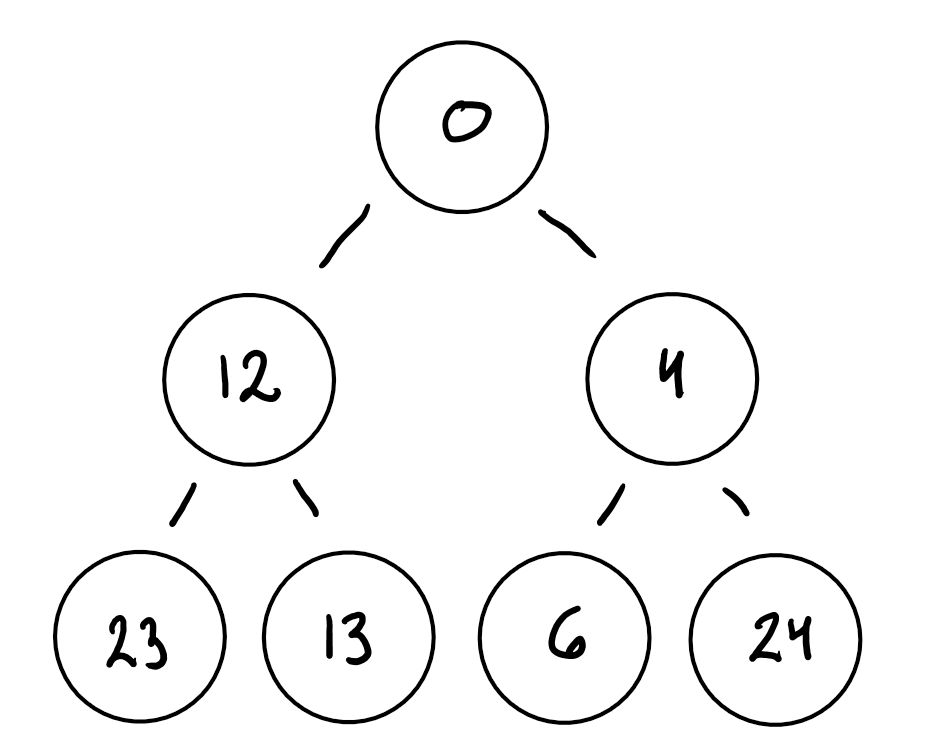
\includegraphics[scale=0.4]{Images/P1A1.PNG}
    \end{center}
    {\tt [8, 11, 8, 12, 14, 9, 10]} is a min-heap.
    \begin{center}
        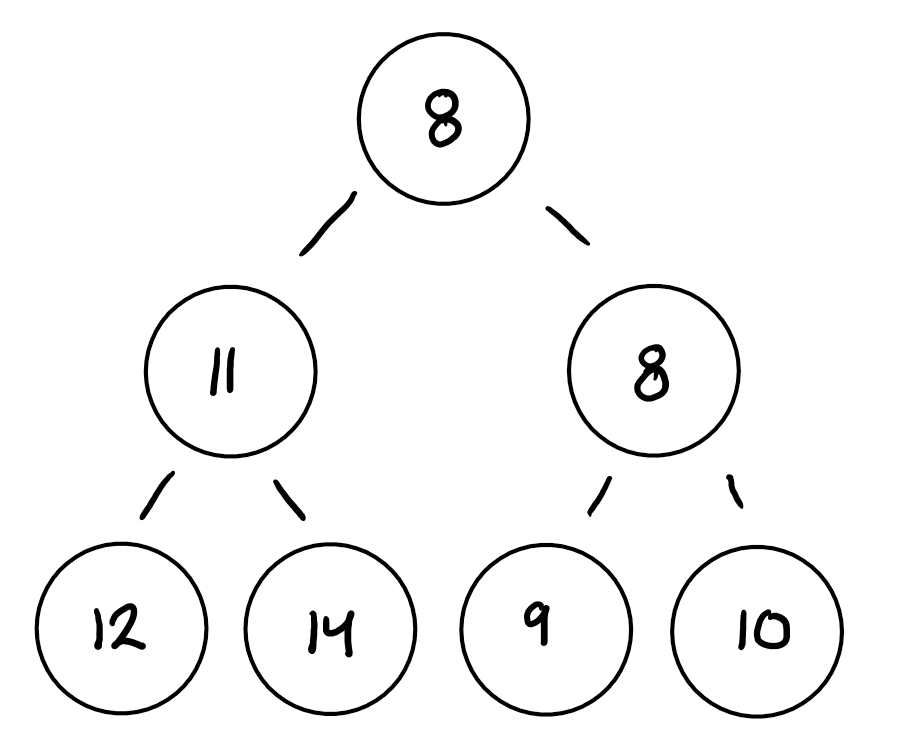
\includegraphics[scale=0.4]{Images/P1A2.PNG}
    \end{center}
    {\tt [23, 7, 16, 4, 7, 12, 1]} is a max-heap.
    \begin{center}
        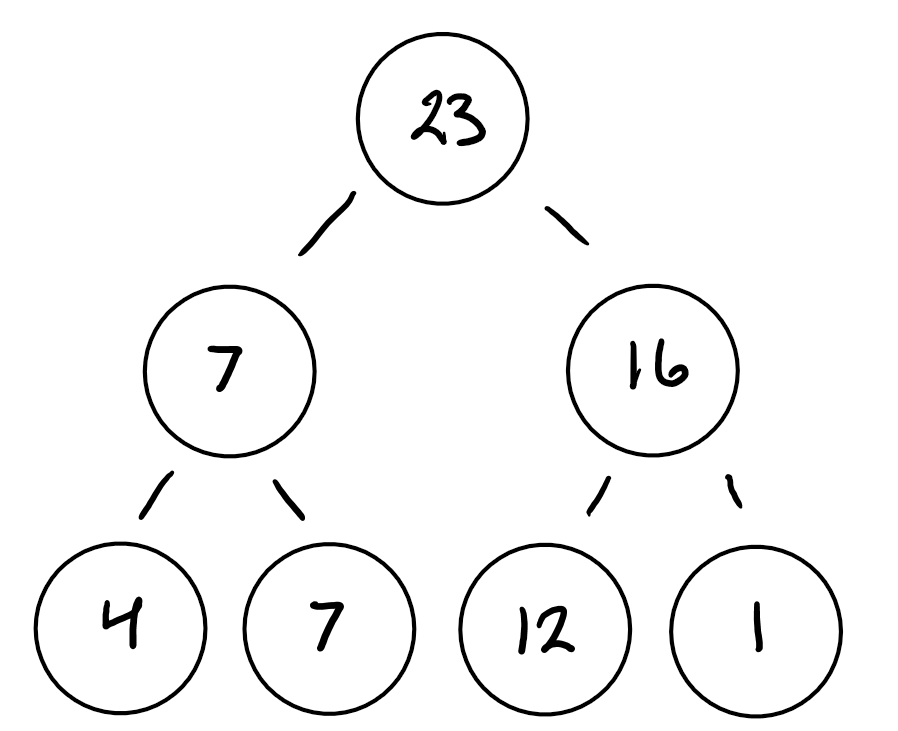
\includegraphics[scale=0.4]{Images/P1A3.PNG}
    \end{center}
    {\tt [9, 6, 10, 2, 7, 4, 11]} is neither a min- nor max-heap.
    \begin{center}
        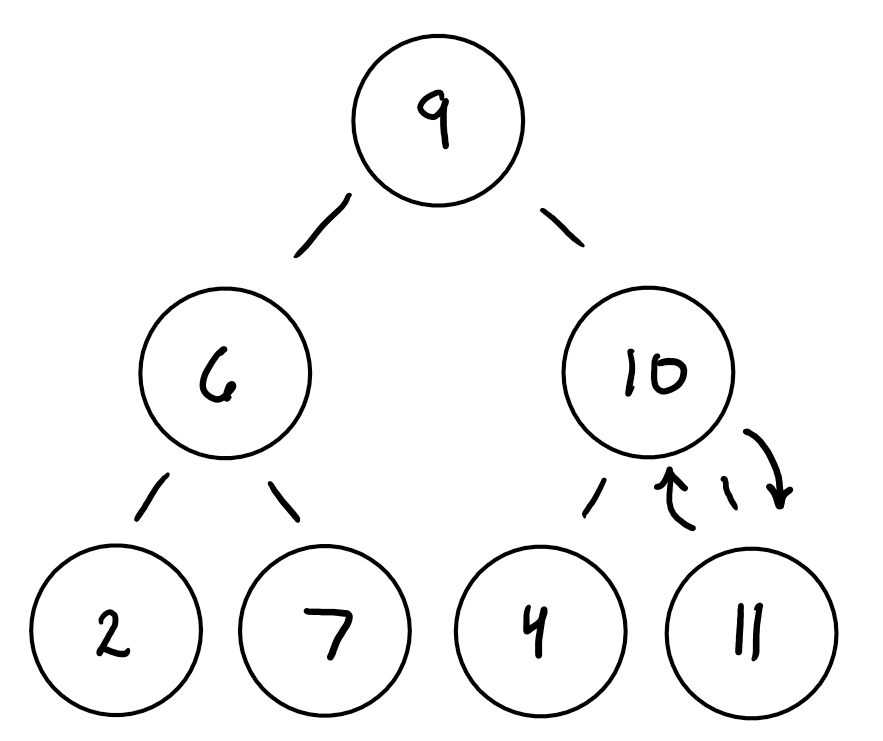
\includegraphics[scale=0.4]{Images/P1A4i.PNG}
        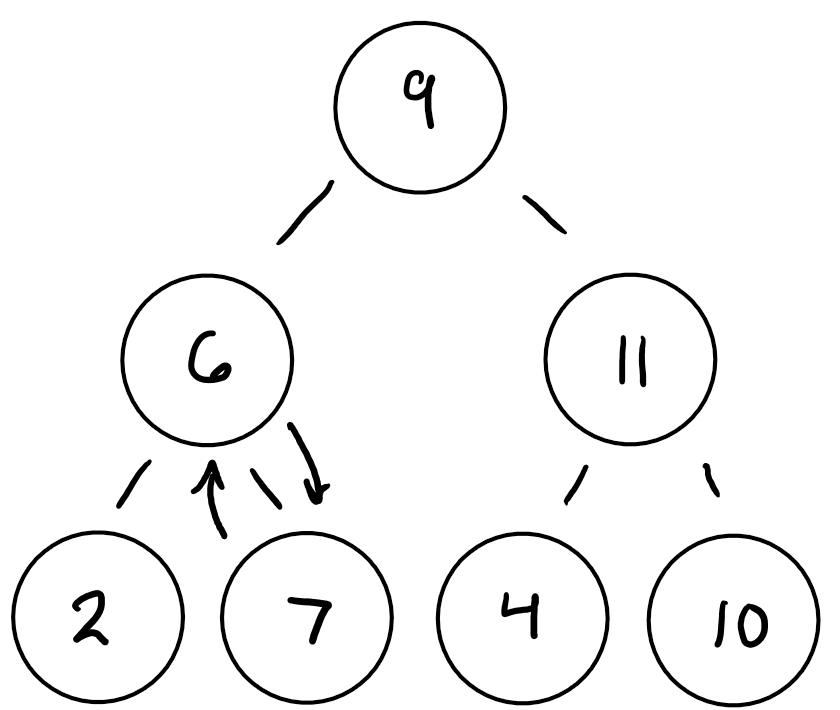
\includegraphics[scale=0.4]{Images/P1A4ii.PNG}
    \end{center}
    \begin{center}
        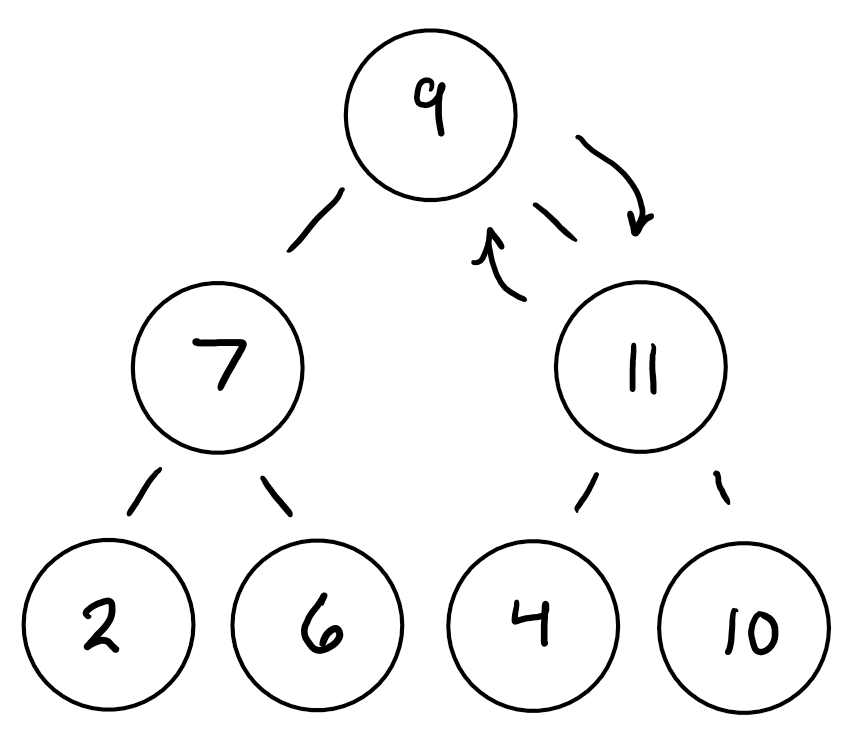
\includegraphics[scale=0.4]{Images/P1A4iii.PNG}
        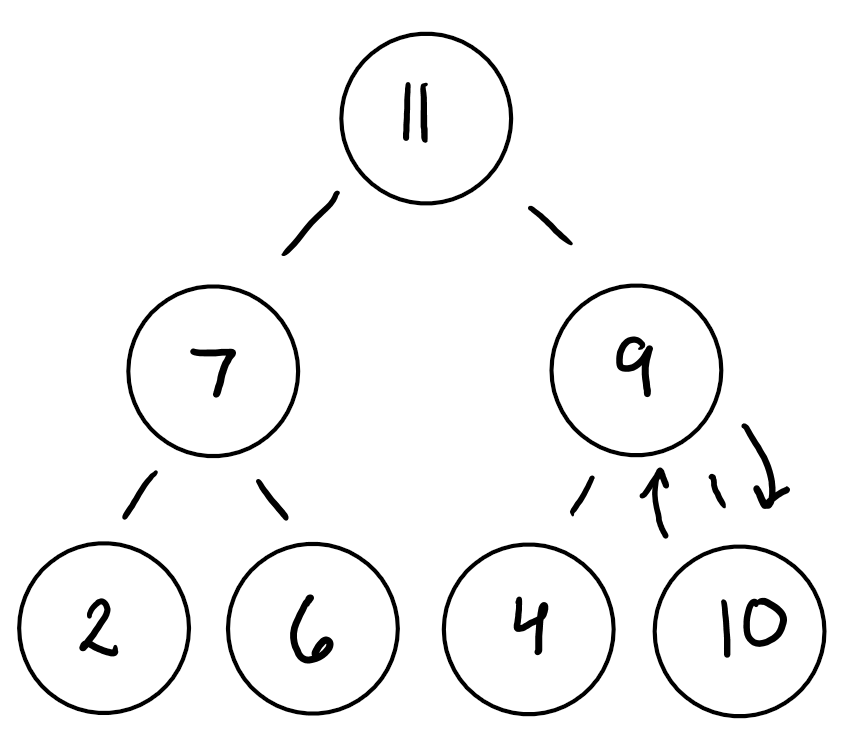
\includegraphics[scale=0.4]{Images/P1A4vi.PNG}
    \end{center}
    \begin{center}
        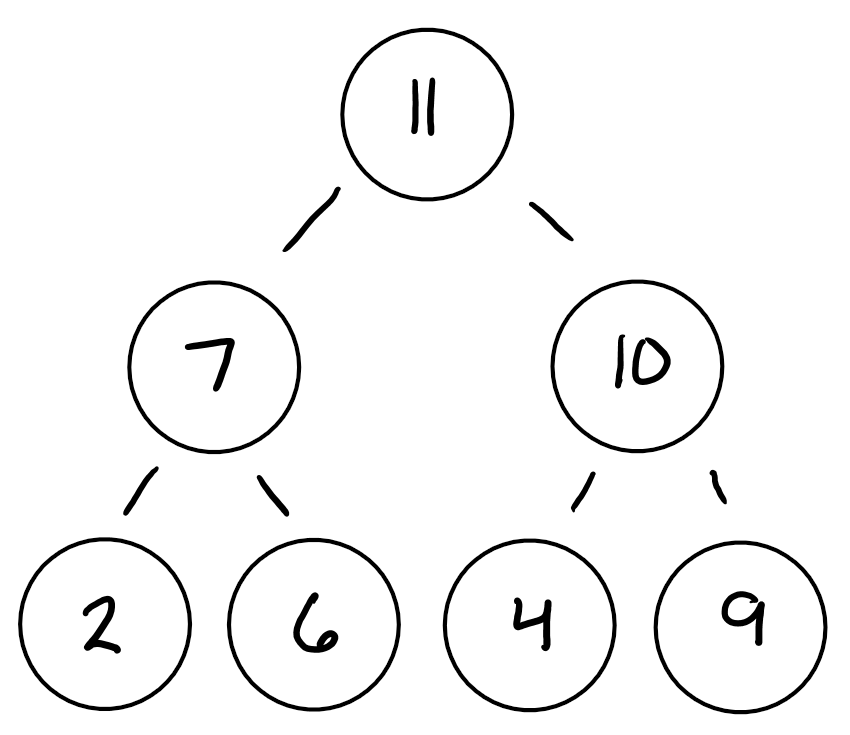
\includegraphics[scale=0.4]{Images/P1A4v.PNG}
    \end{center}
    {\tt [10, 2, 9, 0, 1, 8, 7]} is a max-heap.
    \begin{center}
        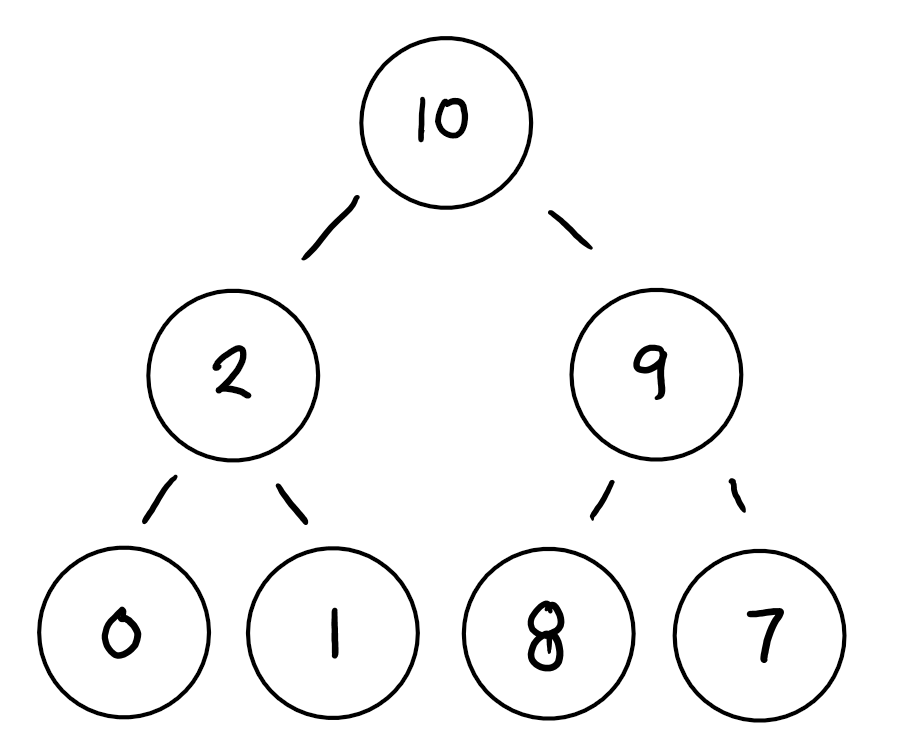
\includegraphics[scale=0.4]{Images/P1A5.PNG}
    \end{center}
\problempart The following lists the possible nodes that can contain the
values of $ k \in K $,
    \begin{enumerate}
        \item $ A $
        \item $ B, C $
        \item $ B, C, D, E, F, G $
        \item $ B, C, D, E, F, G $
        \item $ B, C, D, E, F, G $
        \item $ D, E, F, G $
        \item $ D, E, F, G $
    \end{enumerate}
\problempart {\bf Description} First, the second largest element in the
    max-heap needs to be located. Since the root of the tree representing the
    heap must be the maximum element, then second largest value must be one
    of the children of the root, which ever is larger. If the new value of
    the second largest is greater than the old value, set the second largest
    and call {\tt max\_heapify\_up()} on the element. If the new value of the
    second largest is less than the old value, set the second largest and
    call {\tt max\_heapify\_down()} on the element.

    \smallbreak

    {\bf Correctness} The second largest (non-unique) element has to be one
    of the descendants of the root given that $ A $ is a max-heap. Therefore,
    all the descendants are less than or equal to the root. Furthermore, the
    second largest (non-unique) element must be in the top two levels of the
    heap because it must be greater than or equal to every element except the
    root. Therefore, the (non-unique) second largest must be one of the two
    children of the root, whichever is larger.

    Once the element is set, there are three cases to consider
    \begin{enumerate}
        \item The new value is equal to the old.
        \item The new value is larger than the old.
        \item The new value is less than the old.
    \end{enumerate}

    In the first case, there is no further action to be taken given that the
    max-heap hasn't changed.

    In the second case, let the left and right children of the root be $ c_L
    $ and $ c_R $, respectively. WLOG, assume that $ c_L $ was the second
    largest and has been changed to a new value $ v $ such that $ v > c_L $.
    Since $ c_R $ is unchanged, it must still maintain the max-heap property
    with all of its descendants. Also, since $ v > c_L $, the new tree formed
    under $ v $ must also maintain the max-heap property as $ c_L $ was
    greater than all of its descendants and $ v > c_L $. Thus, the only
    element that could violate the max-heap property is the root. Thus, {\tt
    max\_heapify\_up()} can be called to fix the heap.
    
    In the second case, let the left and right children of the root be $ c_L
    $ and $ c_R $, respectively. WLOG, assume that $ c_L $ was the second
    largest and has been changed to a new value $ v $ such that $ v < c_L $.
    Since $ c_R $ is unchanged, it must still maintain the max-heap property
    with all of its descendants. Also, since $ v < c_L $ and $ c_L $ must be
    less that the root, given it was a max-heap, the root and its children
    (not descendants) must also still satisfy the max-heap property. The only
    elements out of place are $ v $ and possibly all its descendants.
    Therefore, calling {\tt max\_heapify\_down()} will fix the heap.

    \smallbreak

    {\bf Running Time} To find the second largest element only involves
    arithmetic and can be done in $ O(1) $ work. Setting the new value
    involves constant index-lookup, therefore $ O(1) $ work. If the new and
    old values are equal, there is no necessary further work. If the new
    value is greater than the old value, only at worst one swap in {\tt
    max\_heapify\_up()} is required as the height of the tree is $ 1 $. If
    the new value is less than the old value, then {\tt max\_heapify\_down()}
    will require at worst $ O(\log n) $ work. (Slightly less because there is
    one fewer level.) Therefore, the overall running time is $ O(\log n) $.

\end{problemparts}

\newpage
\problem

\begin{problemparts}
\problempart {\bf Description} This data structure will have three
    properties:
    \begin{itemize}
        \item {\tt heaviest\_species}: This will contain the species of the
        heaviest fish that has been caught so far.
        \item {\tt max\_weight}: This will contain the heaviest recorded
        weight of all the fish caught so far.
        \item {\tt weight\_species\_tuples}: This will be a linked list of
        tuples that represent the weight and species of every fish caught.
    \end{itemize}
    This data structure will have two methods:
    \begin{itemize}
        \item {\tt get\_heaviest\_species()}: This will return the value
        stored in \\
        {\tt heaviest\_species}.
        \item {\tt record\_fish(weight, species)}: This will add a new
        linked list node to the front of {\tt weight\_species\_tuples} and
        check if the newly added weight is larger than {\tt max\_weight}. If
        so, {\tt max\_weight} and {\tt heaviest\_species} will be updated
        accordingly.
    \end{itemize}

    \smallbreak

    {\bf Correctness} 
    \begin{itemize}
        \item {\tt record\_fish()}: Given the recording of fish is simply a
        call to a linked list insert-left, the correctness of this operation
        rests on the correctness of linked list insert-right, which is
        assumed to be correct.
        \item {\tt get\_heaviest\_species()}: Since the weight of a new fish
        is always compared to the old maximum weight, which is then updated
        accordingly, it is impossible to add a fish with a weight greater
        than max weight. Additionally, since the heaviest species is updated
        alongside the maximum weight, it will always maintain the species of
        the heaviest fish. Thus, the heaviest species can be returned
        correctly.
    \end{itemize}

    \smallbreak

    {\bf Running Time} 
    \begin{itemize}
        \item {\tt record\_fish()}: To record the new fish, a call to a
        linked list insert-left, which is $ O(1) $, and only a few other
        constant-time updates are made. Therefore, this is a total of $ O(1) $.
        \item {\tt get\_heaviest\_species()}: To return the heaviest species,
        only a stored value is returned requring $ O(1) $ work.
    \end{itemize}

\problempart {\bf Description} This data structure should have one property:
    \begin{itemize}
        \item {\tt fish\_heap}: This is a binary max-heap that stores tuples
        of weights and species of every fish recorded. The key is given by
        the weights of the fish.
    \end{itemize}
    This data structure should have three methods:
    \begin{itemize}
        \item {\tt get\_heaviest\_species()}: This returns the species of the
        maximum element (given by weight) in the binary max-heap {\tt
        fish\_heap}.
        \item {\tt record\_fish(weight, species)}: This inserts an element into
        the binary max-heap {\tt fish\_heap}.
        \item {\tt pop\_heaviest\_fish()}: This finds the max fish (given by
        weight) in {\tt fish\_heap}, returns it, and then removes it.
    \end{itemize}

    \smallbreak

    {\bf Correctness}
    \begin{itemize}
        \item {\tt get\_heaviest\_species()}: This relies on the operation
        find-max in a binary max-heap, which is assumed correct, and
        returning the species property of the returned element which must've
        been set during the record process.
        \item {\tt record\_fish(weight, species)}: This relies on the
        operation insert of a weight-species tuple in a binary max-heap,
        which is assumed correct, sorted based on the weight.
        \item {\tt pop\_heaviest\_fish()}: This relies on the find-max and
        delete-max operations in a binary max-heap, which are assumed
        correct.
    \end{itemize}

    \smallbreak

    {\bf Running Time}
    \begin{itemize}
        \item {\tt get\_heaviest\_species()}: Find-max in a binary max-heap
        is done in $ O(1) $ work.
        \item {\tt record\_fish(weight, species)}: Insert into a binary max
        heap is done in $ O(\log n) $ work.
        \item {\tt pop\_heaviest\_fish()}: Find-max and delete-max in a
        binary max-heap are each $ O(1) $ and $ O(\log n) $, respectively.
    \end{itemize}

\problempart {\bf Description} This data structure should have two properties:
    \begin{itemize}
        \item {\tt lighter\_fish}: This is a max-heap that holds tuples
        containing the weight and species of the lighter half of fish caught.
        \item {\tt heavier\_fish}: This is a min-heap that holds tuples
        containing the weight and species of the heavier half of fish caught.
    \end{itemize}
    This data structure should have five methods:
    \begin{itemize}
        \item {\tt get\_median\_species()}: This calls {\tt find\_median()}
        and returns the species of the median.
        \item {\tt record\_fish(weight, species)}: This calls {\tt
        find\_median()} and if the weight of the new fish is greater, the
        fish is inserted into the min-heap {\tt heavier\_fish}. If the weight
        of the new fish is less, the fish is inserted into the max-heap {\tt
        lighter\_fish}. {\tt rebalance()} is then called to maintain the
        relative sizes of the min and max heaps.
        \item {\tt pop\_median\_fish()}: This calls {\tt find\_median()} and
        returns the value and calls the delete method on the appropriate heap
        given the result of {\tt find\_median()}. To maintain the equal
        halves, {\tt rebalance()} is then called.
        \item {\tt rebalance()}: This method checks if the min- and max-heaps
        are equal in size (give or take 1). If they are not, the min or max
        of the larger is popped and inserted into the other heap.
        \item {\tt find\_median()}: This method returns $ 0 $ if the median
        is minimum of the min-heap and $ 1 $ if the median is the maximum of
        the max-heap. This is determined by the relative sizes of the heaps.
        If one is larger, that one contains the median at the root. If they
        are equal in size, I choose to return the lesser value (or the one
        contained in the max-heap).
    \end{itemize}

    \smallbreak

    {\bf Correctness}
    \begin{itemize}
        \item {\tt get\_median\_species()}: Given the median is kept in the
        min or max of the respective heap, assured by the rebalance method
        argued below, and the find median correctly returns the location, as
        argued below, the median is guaranteed to be found correctly. The
        find-min/max operation on the heap is assumed correct.
        \item {\tt record\_fish(weight, species)}: Since the median is
        correctly located by find-median (argued below) and the value is
        correctly returned by find-min/max in a heap (assumed) then lesser
        and greater halves of the data are maintained if the value greater is
        inserted into the greater half or the value lesser is inserted into
        the lesser half. Rebalancing correctly maintains that the median is
        the min/max of the appropriate heap.
        \item {\tt pop\_median\_fish()}: Given the median is kept in the min
        or max of the respective heap, assured by the rebalance method argued
        below, and the find median correctly returns the location, as argued
        below, the median is guaranteed to be found correctly. The
        find-min/max and delete-min/max operations on a heap are assumed
        correct.
        \item {\tt rebalance()}: If the sizes become unequal, the max of the
        lesser or the min of the greater no longer represents the median. To
        fix this, the data split needs to be shifted towards the greater half
        to restore balance. If the lesser half is larger, the maximum element
        should really be the minimum of the greater half. Therefore a delete
        from the lesser and insert into the greater will do this. And vice
        versa for if the greater halve is larger. Therefore, this maintains
        the median in the min/max of the heap.
        \item {\tt find\_median()}: Since the median is middle value of
        sorted data, it must either be the maximum of the lesser half or the
        minimum of the upper half. If the halves are unequal, the greater one
        must contain the median. Therefore, this will return the location of
        the median correctly. If the halves are equal, my choice is just to
        return the lesser of the two.
    \end{itemize}

    \smallbreak

    {\bf Running Time}
    \begin{itemize}
        \item {\tt get\_median\_species()}: This finds the median ($O(1)$ as
        argued below) and then calls a find-min/max on a heap which is also $
        O(1) $. Therefore, the overall work is $ O(1) $.
        \item {\tt record\_fish(weight, species)}: This finds the location of
        median, which is $ O(1) $ as argued below, and then calls a
        find-min/max on a heap, which is $ O(\log n) $. No matter the result
        of the comparison, an insert to a heap is called which is $ O(\log n) $.
        Then, rebalancing is needed, taking $ O(\log n) $ as argued below.
        Therefore, the total work is $ O(\log n ) $.
        \item {\tt pop\_median\_fish()}: This finds the location of median,
        which is $ O(1) $ as argued below, and then calls a find-max/min on a
        heap, which is also $ O(1) $. Then, the element is deleted from the
        heap which takes $ O(\log n) $. Lastly, rebalancing takes place which
        is $ O(\log n) $ as argued below. Therefore, overall work is $ O(\log
        n) $.
        \item {\tt rebalance()}: The size comparison takes $ O(1) $
        (assuming, once again, that this is a property of the heap). If the
        sizes differ by more than one, a delete max/min is called on a heap
        (requiring $ O(\log n) $) and a subsequent insert on a heap
        (requiring $ O(\log n) $). Therefore, the total work is $ O(\log n) $.
        \item {\tt find\_median()}: This only compares the relative sizes of
        (which I will assume is stored in the heap, if not, it is easy to
        implement), which takes $ O(1) $.
    \end{itemize}

\problempart {\bf Description} This data structure should have one property:
    \begin{itemize}
        \item {\tt fish}: This is a min-heap that contains the fish that are
        caught during the trip.
    \end{itemize}
    This data structure should have two methods:
    \begin{itemize}
        \item {\tt add\_fish(weight, species)}: This method will insert the
        newest caught fish into the {\tt fish} heap. This assumes that
        Frankie is responsible for calling {\tt identify\_discard()} to
        determine both if a fish should be discarded and which fish to remove
        after catching the last fish.
        \item {\tt identify\_discard()}: If the size of the heap is less than
        or equal to $ k $, this method will return {\tt None} as no fish
        needs to be removed. If the heap is greater than $ k $, this method
        will find the minimum fish within the {\tt fish} heap and return it.
        This assumes that frankie has some other means of removing the fish as
        this method will not remove the fish, just identify it.
    \end{itemize}

    \smallbreak

    {\bf Correctness} For each operation
    \begin{itemize}
        \item {\tt add\_fish(weight, species)}: This is a simple call to an
        insert operation on a min-heap. This is assumed correct.
        \item {\tt identify\_discard()}: If the number of fish caught is less
        than or equal to the capacity, this is certainly correct as no fish
        will be identified to be removed. If the number of fish is greater
        than the size of the capacity, then the lightest fish will be
        identified. This is done through a find-min operation on a min-heap
        which is assumed correct.
    \end{itemize}
    This also guarantees that Frankie will end up with the largest fish he
    caught during the entire trip as there was no way for Frankie to have
    thrown out a fish larger than the $ k $ he had at the end of his trip.

    \smallbreak

    {\bf Running Time}
    \begin{itemize}
        \item {\tt add\_fish(weight, species)}: This is a simple call to an
        insert operation on a min-heap known to be $ O(\log n) $.
        \item {\tt identify\_discard()}: Involves constant-time size
        comparison (assuming the size of the heap is a property, easy to
        implement) and a find-min on a heap which is known to be $ O(1) $.
        Assuming no remove is performed, this operation has a total of $ O(1)
        $ work. If the remove is performed also, a call to delete-min on a
        min-heap will be called which is $ O(\log n ) $ and then the total
        work would be $ O(\log n)$.
    \end{itemize}

\end{problemparts}

\newpage
\problem

\begin{problemparts}
\problempart Consider the bottom-up/iterative implementation of insertion
    sort. Let $ A $ be an unsorted, $ k $-proximate array. Insertion sort
    slowly expands a sorted subsection of the array $ A $ located at the
    beginning of $ A $. Let this sorted subsection be from $ a_0 $ to $ a_j
    $. Then, $ a_{j + 1} $ is compared with $ a_j $ and swapped if out of
    order. Then, $ a_j $ is compared with $ a_{j - 1} $ and swapped if out of
    order, and so on until $ a_1 $ is compared with $ a_0 $. This approaches
    $ O(n) $ swaps. However, given that $ a_{j} $ can only be at most $ k $
    slots away from its final sorted position $ a_i $, swaps do not need to
    occur beyond $ a_i $ as $ a_j $ must be located there or somewhere
    earlier. Therefore, at maximum, only $ k $ swaps are needed. Since the
    number of iterations is $ n $ and each iteration will perform at most $ k
    $ swaps, this must be $ O(kn) $.
\problempart {\bf Description} I will use a modified definition of a min-heap
    to aid in the implementation of {\tt proximate\_sort()}. This heap will
    have two properties:
    \begin{itemize}
        \item {\tt k}: This is the size of the heap.
        \item {\tt arr}: This is the fixed (non-dynamic) array containing the
        elements of the heap.
    \end{itemize}
    And also three methods:
    \begin{itemize}
        \item {\tt init(A, k)}: This will set {\tt k } and allocate {\tt
        arr}. Then it will call {\tt min\_heapify\_up()} after inserting each
        of the $ k $ members of $ A $. (There is a faster way, but since the
        input was given as a tuple, I can't perform an in-place heapify.)
        \item {\tt swap\_top(x)}: This will set the root value as $ x $ and
        call {\tt min\_heapify\_down()} on the new element. Then it will
        return the old root value.
        \item {\tt pop()}: This will return the root value and remove it,
        calling {\tt min\_heapify\_down()} afterwards.
    \end{itemize}
    Now, the actual algorithm {\tt proximate\_sort()} will initialize the heap
    with the first $ k + 1 $ elements of $ A $. Then, for each element after
    the first $ k + 1 $, it will call {\tt swap\_top()} and push the returned
    element to the sorted output. Once this loop completes, the remaining
    elements in the heap are {\tt pop()}'ed off and pushed into the sorted
    output. The sorted output is then returned.

    \smallbreak

    {\bf Correctness}

    \smallbreak

    {\bf Running Time} For the methods in the data structure
    \begin{itemize}
        \item {\tt init(A, k)}: Allocation requires $ O(k) $, and for each of
        the $ k $ elements, min-heapify requires $ O(\log k) $ work.
        Therefore, total work is $ O(k + k \log k) \in O( k \log k) $. (Once
        again, this could be simplied if an in-place sort were possible, i.e.
        not supplying tuples.)
        \item {\tt swap\_top(x)}: A single call to min-heapify is used which
        is $ O(\log k) $.
        \item {\tt pop()}: A single call to min-heapify is used which is $
        O(\log k) $.
    \end{itemize}
    Then, the proximate-sort algorithm will make one call to the
    initialization method which is $ O(k \log k) $, $ n - k $ calls to the
    swap method which is $ O(\log k) $, and $ k $ calls to the pop method
    which is $ O(\log k) $. Therefore, total work is $ O(n \log k) $.

\problempart Submit your implementation to {\small\url{alg.mit.edu/PS3}}
\end{problemparts}

\end{problems}

\end{document}

